\let\negmedspace\undefined
\let\negthickspace\undefined
\documentclass[journal]{IEEEtran}
\usepackage[a5paper, margin=10mm, onecolumn]{geometry}
\usepackage{tfrupee}

\setlength{\headheight}{1cm}
\setlength{\headsep}{0mm}

\usepackage{gvv-book}
\usepackage{gvv}
\usepackage{cite}
\usepackage{amsmath,amssymb,amsfonts,amsthm}
\usepackage{algorithmic}
\usepackage{graphicx}
\usepackage{textcomp}
\usepackage{xcolor}
\usepackage{txfonts}
\usepackage{listings}
\usepackage{enumitem}
\usepackage{mathtools}
\usepackage{gensymb}
\usepackage{comment}
\usepackage[breaklinks=true]{hyperref}
\usepackage{tkz-euclide}
\usepackage{listings}
\def\inputGnumericTable{}
\usepackage[latin1]{inputenc}
\usepackage{color}
\usepackage{array}
\usepackage{longtable}
\usepackage{calc}
\usepackage{multirow}
\usepackage{hhline}
\usepackage{ifthen}
\usepackage{lscape}

\begin{document}

\bibliographystyle{IEEEtran}
\vspace{3cm}

\title{5.3.37}
\author{EE25BTECH11003 - Adharvan Kshathriya Bommagani}
{\newpage\maketitle}

\renewcommand{\thefigure}{\theenumi}
\renewcommand{\thetable}{\theenumi}
\setlength{\intextsep}{10pt}

\textbf{Question}:\\
Draw the graphs of the following equations
\begin{center}
    

    3x - 4y + 6 = 0 \\
    3x + y - 9 = 0
\end{center}
Also, determine the co-ordinates of the vertices of the triangle formed by these lines and the X axis.

\bigskip

\textbf{Solution}:\\

The triangle is formed by the intersection of three lines:
\begin{align}
    L_1: \myvec{3 \\ -4}^\top \myvec{x \\ y} = -6 \\
    L_2: \myvec{3 \\ 1}^\top \myvec{x \\ y} = 9 \\
    L_3: \myvec{0 \\ 1}^\top \myvec{x \\ y} = 0
\end{align}
The vertices, which we will call $\vec{A}$, $\vec{B}$, and $\vec{C}$, are the intersection points of these lines. We solve for them using Gaussian elimination (row reduction).

\bigskip

\textbf{Vertex $\vec{A}$: Intersection of $L_1$ and $L_2$} \\
The system is: $3x - 4y = -6$ and $3x + y = 9$. \\
The augmented matrix is:
\begin{align}
    \myaugvec{2}{
        3 & -4 & -6 \\
        3 & 1 & 9
    }
\end{align}

Apply the row operation $R_2 \to R_2 - R_1$:
\begin{align}
    \myaugvec{2}{
        3 & -4 & -6 \\
        0 & 5 & 15
    }
\end{align}
From the second row, $5y = 15 \implies y=3$. Substituting into the first row ($3x - 4y = -6$), we get:
\begin{align}
    3x - 4(3) = -6 \implies 3x - 12 = -6 \implies 3x = 6 \implies x=2.
\end{align}
\begin{align}
    \vec{A}=\myvec{2 \\ 3}
\end{align}

\bigskip

\textbf{Vertex $\vec{B}$: Intersection of $L_1$ and $L_3$} \\
The system is: $3x - 4y = -6$ and $y = 0$. \\
The augmented matrix is:
\begin{align}
    \myaugvec{2}{
        3 & -4 & -6 \\
        0 & 1 & 0
    }
\end{align}
This matrix is already in row-echelon form. From the second row, $y=0$. Substituting into the first row ($3x - 4y = -6$), we get:
\begin{align}
    3x - 4(0) = -6 \implies 3x = -6 \implies x=-2.
\end{align}
\begin{align}
    \vec{B}=\myvec{-2 \\ 0}
\end{align}



\textbf{Vertex $\vec{C}$ : Intersection of $L_2$ and $L_3$} \\
The system is: $3x + y = 9$ and $y = 0$. \\
The augmented matrix is:
\begin{align}
    \myaugvec{2}{
        3 & 1 & 9 \\
        0 & 1 & 0
    }
\end{align}
This matrix is in row-echelon form. From the second row, $y=0$. Substituting into the first row ($3x + y = 9$), we get:
\begin{align}
    3x + 0 = 9 \implies 3x = 9 \implies x = 3.
\end{align}
\begin{align}
    \vec{C}=\myvec{3 \\ 0}
\end{align}



The coordinates of the vertices of the triangle are $\mathbf{(2, 3)}$, $\mathbf{(-2, 0)}$, and $\mathbf{(3, 0)}$.

\newpage

\textbf{Plot of the Lines and Triangle:}
\begin{figure}[H]
    \centering
    % To generate the actual plot, you would use a package like pgfplots or insert an image file.
    % Example using an image file:
    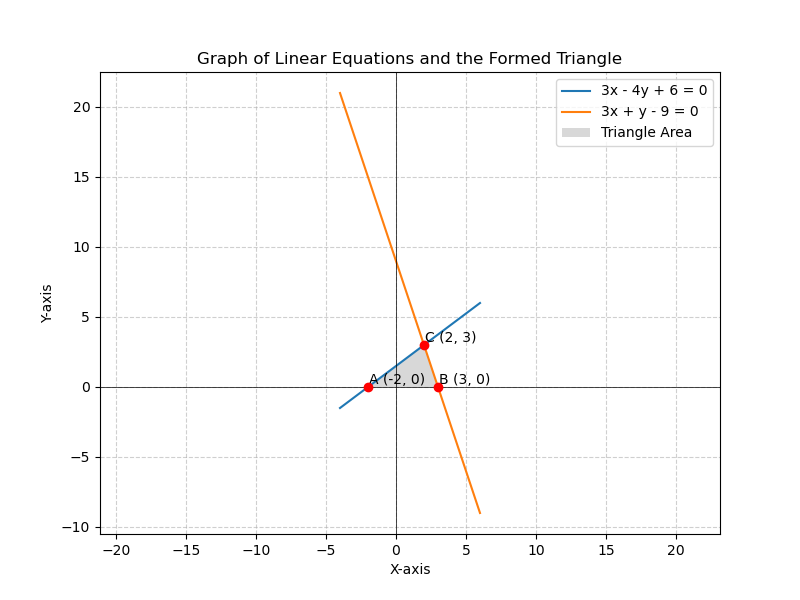
\includegraphics[width=1.1\columnwidth]{figs/fig1.png}
    \caption{figure for 5.3.37}
    \label{fig:triangle}
\end{figure}

\end{document}